\documentclass[11pt,a4paper]{report}
\usepackage[T1]{fontenc}
\usepackage[utf8]{inputenc}
\usepackage{lmodern}
\usepackage{microtype}
\usepackage[a4paper,margin=2.4cm]{geometry}
\usepackage{amsmath,amssymb}
\usepackage{graphicx}
\usepackage{booktabs,longtable,array}
\usepackage{xcolor}
\usepackage{float}
\usepackage{enumitem}
\usepackage{hyperref}
\usepackage{bookmark}
\usepackage{fancyhdr}
\usepackage{caption}
\usepackage[numbers,sort&compress]{natbib}

\graphicspath{{Projeto_Radomes_Multifaixa_Revisado_Markdown/figures/}}
\hypersetup{colorlinks=true,linkcolor=blue!50!black,citecolor=blue!50!black,urlcolor=blue!50!black,pdftitle={Projeto Técnico Completo da Rede de Radomes Multifaixa}}
\setlength{\emergencystretch}{3em}
\setlist{itemsep=2pt,topsep=4pt}
\pagestyle{fancy}
\fancyhf{}
\lhead{Rede de Radomes Multifaixa}
\rhead{Projeto técnico consolidado}
\cfoot{\thepage}
\setlength{\headheight}{14pt}

\newcommand{\radome}{\textsc{Radome}}
\newcommand{\vthree}{\radome V3}
\newcommand{\figref}[1]{Figura~\ref{#1}}
\newcommand{\SI}[2]{\ensuremath{#1\,\mathrm{#2}}}

\title{\textbf{Rede Distribuída de Radomes Conformais Multifaixa e Polarimétricos}\\[0.5em]\large Projeto técnico consolidado para sensoriamento eletromagnético passivo, radiogoniometria e localização multiestática}
\author{Documento técnico de pesquisa, simulação e prototipagem}
\date{Agosto de 2026}

\begin{document}
\maketitle
\begin{abstract}
Este documento consolida os documentos conceituais, arquitetônicos, eletrônicos, de infraestrutura e de revisão de literatura disponíveis no projeto Radome. A proposta descreve uma rede distribuída de radomes geodésicos instalados em sítios elevados, com abertura híbrida, antenas Yagi externas para VHF, antenas menores para UHF e micro-ondas, aquisição polarimétrica, processamento local orientado a eventos, sincronização temporal distribuída e fusão estatística para radiogoniometria, localização e rastreamento. O projeto mantém cadeias próprias por família de antenas e uma interface comum de sincronismo, calibração e fusão; nenhuma precisão operacional pode ser declarada sem orçamento de enlace, calibração e validação de campo.
\end{abstract}

\tableofcontents
\listoffigures

\chapter{Escopo, motivação e estado do projeto}

O projeto propõe uma infraestrutura de vigilância passiva do espectro eletromagnético baseada em múltiplos radomes geodésicos instalados em bases elevadas. Cada estação combina aberturas receptoras, cadeias RF multifaixa, processamento na borda, referência temporal e comunicação óptica. Várias estações podem cooperar para estimar ângulo de chegada (AOA), diferença de tempo de chegada (TDOA), diferença de frequência de chegada (FDOA), Doppler e estado de polarização.

A arquitetura pode utilizar sinais de oportunidade provenientes de radiodifusoras, redes celulares, satélites, transmissores de telecomunicações e outras fontes conhecidas. No caso bistático, a medida de atraso compara o caminho direto de referência com o caminho que passa pelo alvo e chega ao receptor. A rede não deve ser descrita como capaz de ``triangular qualquer energia'': ela precisa associar formas de onda, identificar ou estimar o iluminador e aplicar o modelo de propagação adequado.

O projeto permanece conceitual. Frequências, locais, alcances, probabilidades de detecção e precisão de localização são metas de pesquisa, não garantias operacionais. A validação deve ocorrer por simulação eletromagnética, bancada, câmara anecoica, ensaios ambientais e campanhas externas.

\section{Objetivos}
\begin{itemize}
  \item desenvolver uma arquitetura de recepção passiva multifaixa e polarimétrica;
  \item demonstrar localização cooperativa com três nós VHF/UHF;
  \item medir e controlar atrasos de antena, radome, RF, ADC, clock e fibra;
  \item preservar dados brutos em buffers locais para auditoria e análise posterior;
  \item integrar a plataforma eletromagnética à infraestrutura energética, térmica e de comunicações de montanha.
\end{itemize}

\chapter{Arquitetura geral da rede}

A rede possui três níveis: nós sensores, processamento regional e centro de fusão. Um nó recebe sinais diretos de emissores, sinais emitidos por objetos e sinais refletidos. Os nós transmitem eventos, metadados, espectros e janelas I/Q selecionadas; o fluxo bruto contínuo permanece local salvo em campanhas específicas.

\begin{figure}[H]
\centering
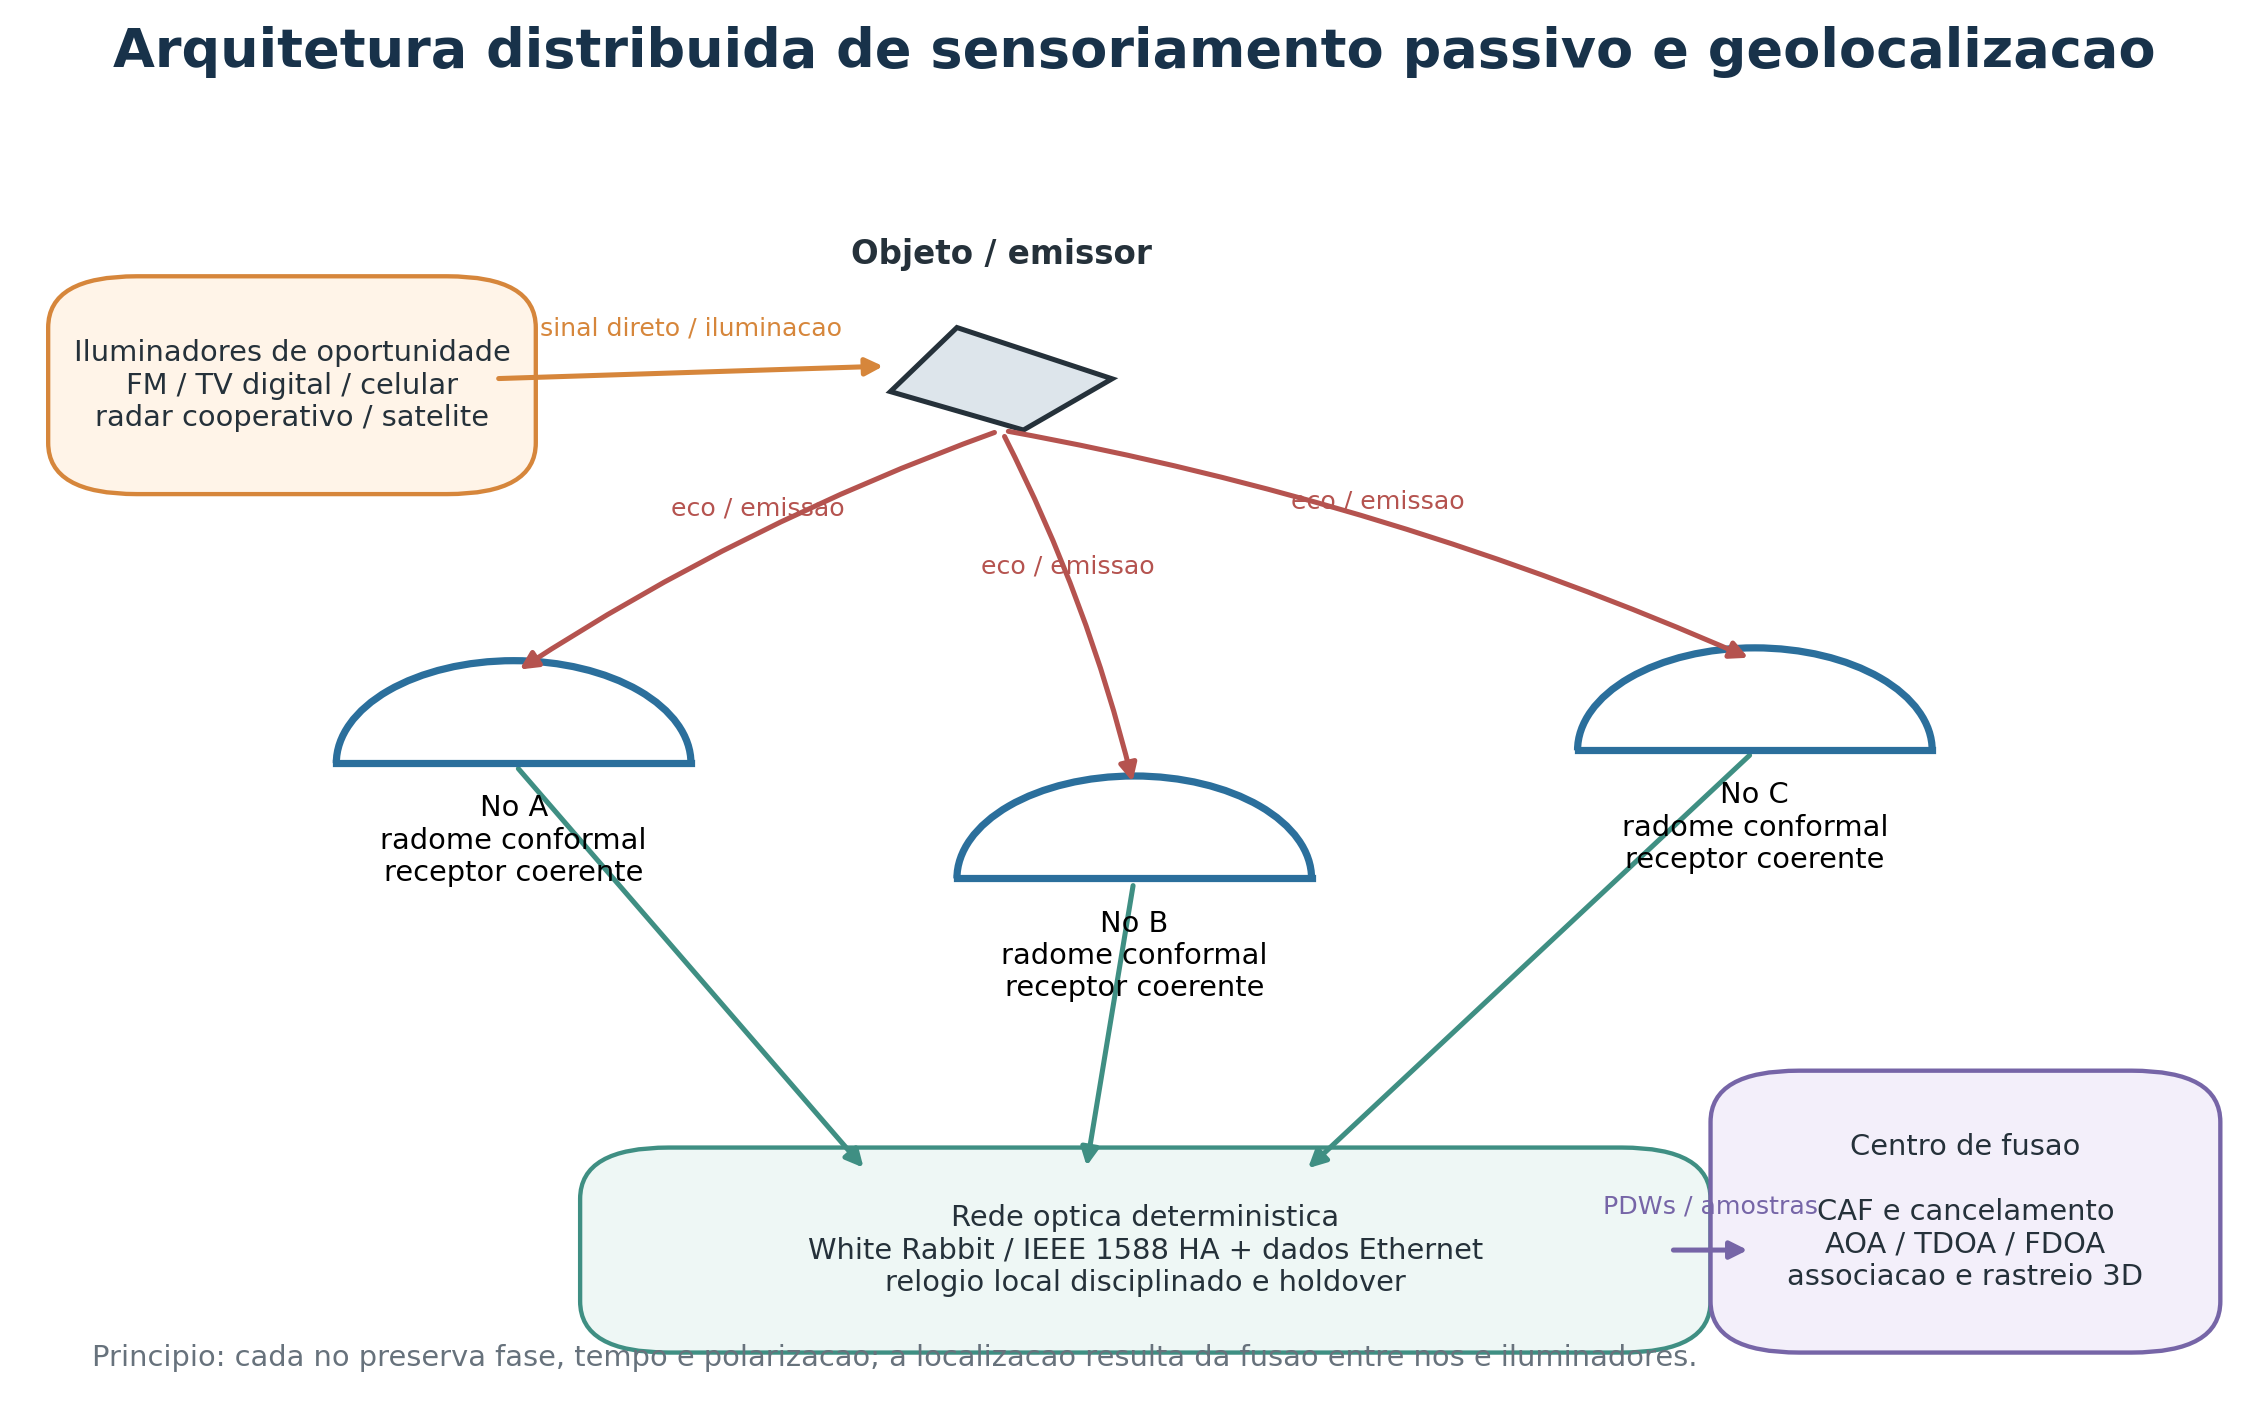
\includegraphics[width=0.96\textwidth]{fig01_arquitetura_rede.png}
\caption{Arquitetura distribuída de iluminadores, objeto, nós receptores, rede de tempo e centro de fusão.}
\label{fig:arquitetura}
\end{figure}

A topologia recomendada é hierárquica. Clusters locais com linhas de base de dezenas de quilômetros atendem alvos de baixa altitude e iluminadores regionais. Clusters regionais ampliam a cobertura. Linhas de base muito longas podem ser úteis para HF, objetos espaciais e sinais de alta altitude, desde que exista visada comum e um iluminador compatível.

\section{Planos de comunicação}
\begin{longtable}{p{0.22\textwidth}p{0.42\textwidth}p{0.24\textwidth}}
\toprule
\textbf{Plano} & \textbf{Conteúdo} & \textbf{Característica}\\
\midrule
Tempo e frequência & PPS, ToD, referência, atraso da fibra e estado de sincronismo & determinístico e crítico\\
Dados científicos & eventos, PDWs, espectros, feixes e janelas I/Q & seletivo, com timestamp\\
Gerenciamento & temperatura, energia, alarmes, firmware e calibração & baixa taxa, alta disponibilidade\\
Contingência & pacotes compactados e diagnóstico & tolera latência; não substitui o plano temporal\\
\bottomrule
\end{longtable}

\chapter{Geometria do radome V3}

O \vthree\ parte de um icosaedro regular com $V_0=12$ vértices, $E_0=30$ arestas e $F_0=20$ faces. Cada macroface triangular é subdividida em três faces receptoras por um vértice radializado. O resultado é uma malha fechada com:
\[
V=32,\qquad E=90,\qquad F=60,
\]
e a relação de Euler é verificada por:
\[
V-E+F=32-90+60=2.
\]

Para raio preliminar $R=\SI{3.1445}{m}$, o diâmetro do envelope é $D=2R=\SI{6.2890}{m}$. O raio não deve ser confundido com a altura de uma estrutura fechada. As arestas originais do icosaedro são aproximadamente $\SI{3.3063}{m}$ e as arestas radiais das faces subdivididas aproximadamente $\SI{2.0152}{m}$.

Cada face receptora deve ser tratada como setor mecânico e computacional, não como região eletromagnética isolada. A sobreposição angular entre faces vizinhas é necessária para calibração, interpolação, confirmação espacial e estimação de direção.

\section{Casco e estrutura}

A solução mecânica combina esqueleto triangulado, painéis dielétricos e módulos internos. Uma parede A-sandwich de peles dielétricas e núcleo de baixa densidade é um ponto de partida, mas a espessura deve ser otimizada para múltiplas janelas, incidências TE/TM, chuva, umidade, temperatura e envelhecimento. Fibra de carbono e estruturas metálicas contínuas devem ser evitadas nas aberturas de micro-ondas, salvo quando sua função eletromagnética for deliberadamente modelada.

\chapter{Abertura multifaixa e polarimetria}

A proposta revisada utiliza uma abertura híbrida: uma Yagi externa direcional para VHF, antenas menores e tiles para UHF e micro-ondas, e sensores próprios para HF. Cada família espectral possui elementos, filtros, conversores e taxas de amostragem próprios, integrados pela estrutura e pelos serviços comuns da face.

\begin{figure}[H]
\centering
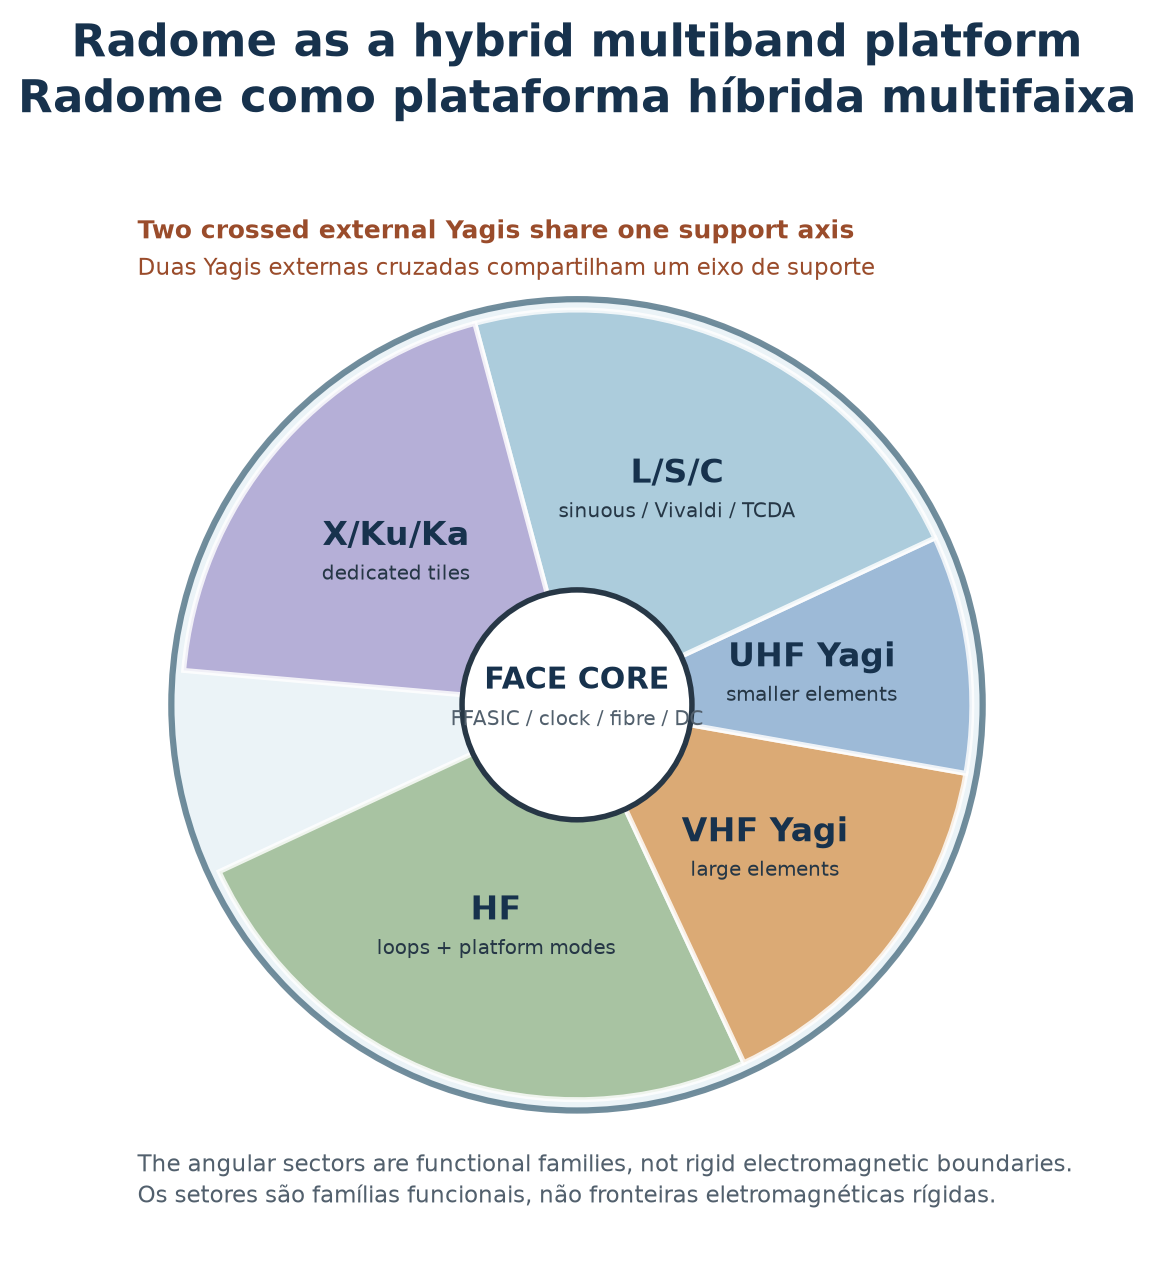
\includegraphics[width=0.98\textwidth]{fig02_zonamento_radome.png}
\caption{Zonamento funcional de uma plataforma quase esférica. As cores representam famílias de subsistemas.}
\label{fig:zonamento}
\end{figure}

\begin{longtable}{p{0.18\textwidth}p{0.36\textwidth}p{0.36\textwidth}}
\toprule
\textbf{Subfaixa} & \textbf{Elementos} & \textbf{Conversão e função}\\
\midrule
HF, 3--30 MHz & loops, dipolos cruzados e excitadores de modos & amostragem direta; AOA por diversidade de padrões e rede\\
VHF, 30--300 MHz & dipolos, loops, log-periódicas e arrays esparsos & pré-seleção e ADC de dezenas ou centenas de MS/s\\
UHF, 0,3--1 GHz & arrays dual-pol, espirais e elementos vetoriais & beamforming por setor e amostragem direta ou IF\\
L/S/C, 1--8 GHz & sinuous, espiral, Vivaldi ou TCDA & DDC após ADC ou downconversion\\
X/Ku, 8--18 GHz & patches, slots ou dipolos acoplados & super-heteródino coerente e varredura eletrônica\\
K/Ka, 18--40 GHz & tiles Rx dual-pol dedicados & conversão local para IF e ADC por sub-banda\\
\bottomrule
\end{longtable}

\begin{figure}[H]
\centering
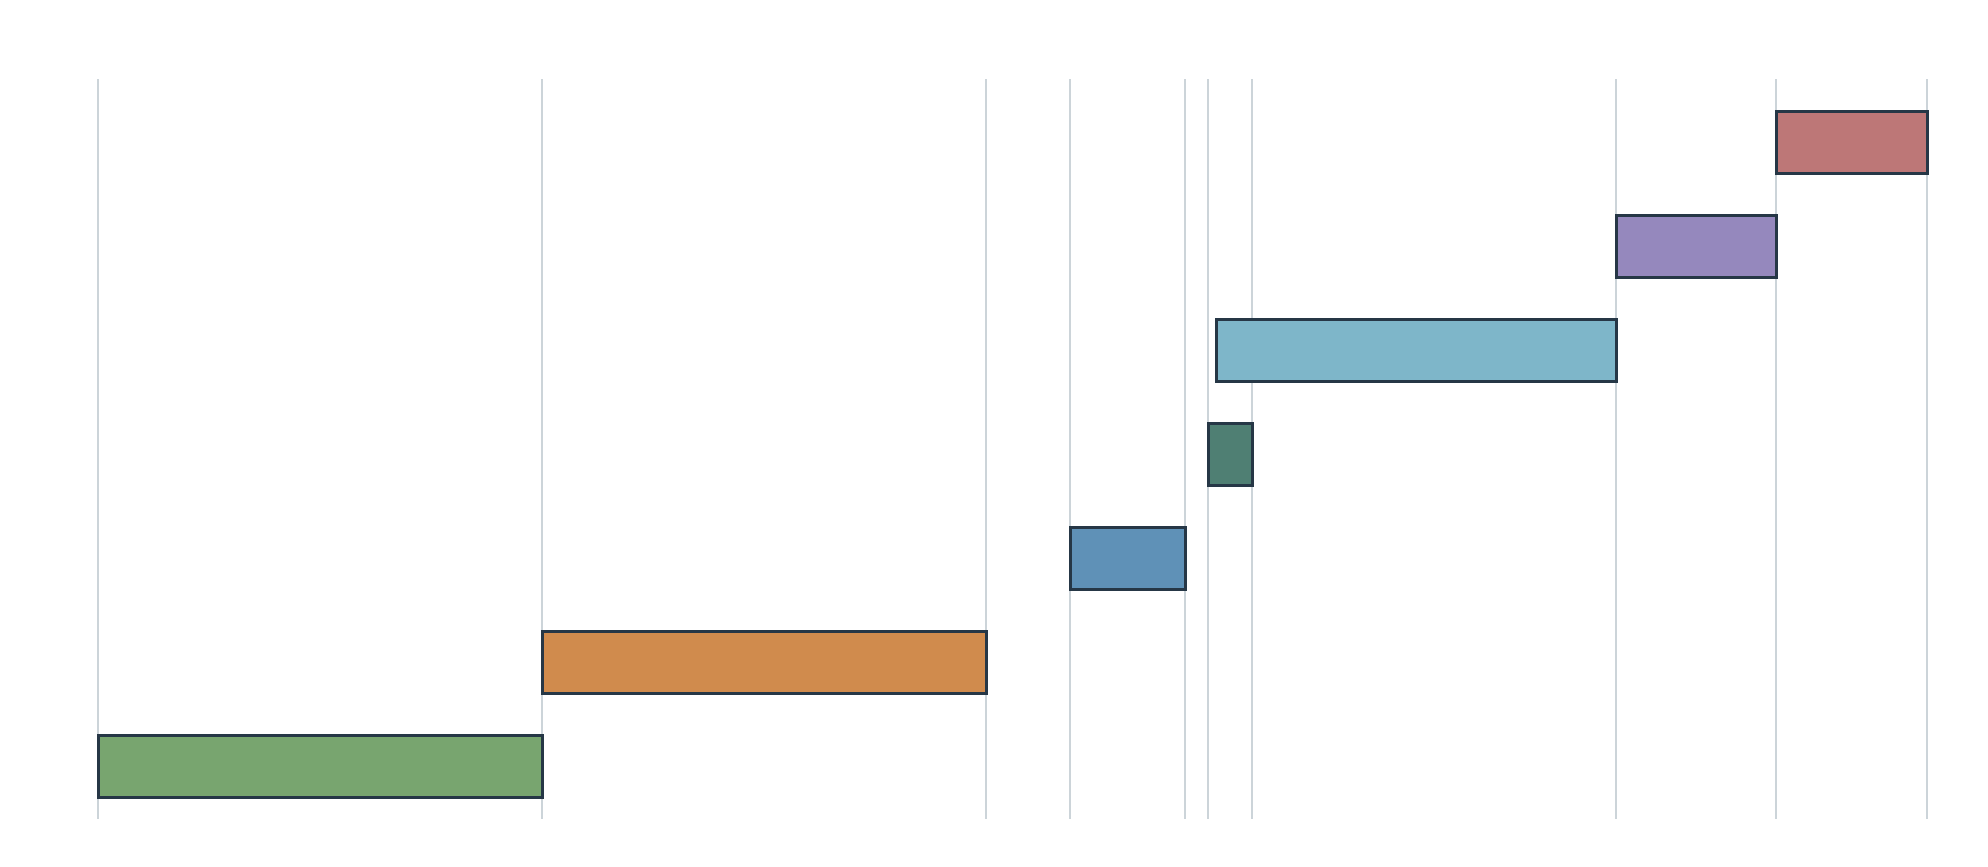
\includegraphics[width=0.98\textwidth]{fig04_particionamento_espectro.png}
\caption{Particionamento recomendado do espectro. A escala logarítmica evidencia a incompatibilidade de uma cadeia única.}
\label{fig:espectro}
\end{figure}

Em HF, uma face de poucos metros é eletricamente pequena, especialmente em 3 MHz, onde $\lambda$ é aproximadamente $\SI{100}{m}$. A direção deve explorar diversidade modal da plataforma, loops, dipolos cruzados e modelos ionosféricos. Em VHF/UHF, um demonstrador com 8 a 24 elementos dual-pol é mais favorável. Em micro-ondas, tiles separados ou aberturas compartilhadas com razões moderadas de frequência são a solução conservadora.

\section{Aquisição vetorial}

Cada elemento relevante deve fornecer duas portas ortogonais coerentes. Em uma base local $x$--$y$, a síntese ideal pode ser escrita como:
\[
E_{\mathrm{RHCP}}=\frac{E_x-jE_y}{\sqrt{2}},\qquad
E_{\mathrm{LHCP}}=\frac{E_x+jE_y}{\sqrt{2}}.
\]
Em uma superfície curva, cada face possui uma base tangencial própria. Os vetores devem ser rotacionados para um sistema comum antes da fusão. O erro de razão axial depende de amplitude, fase, acoplamento e atraso de grupo, portanto a calibração deve ser função de frequência, temperatura e ângulo.

\begin{figure}[H]
\centering
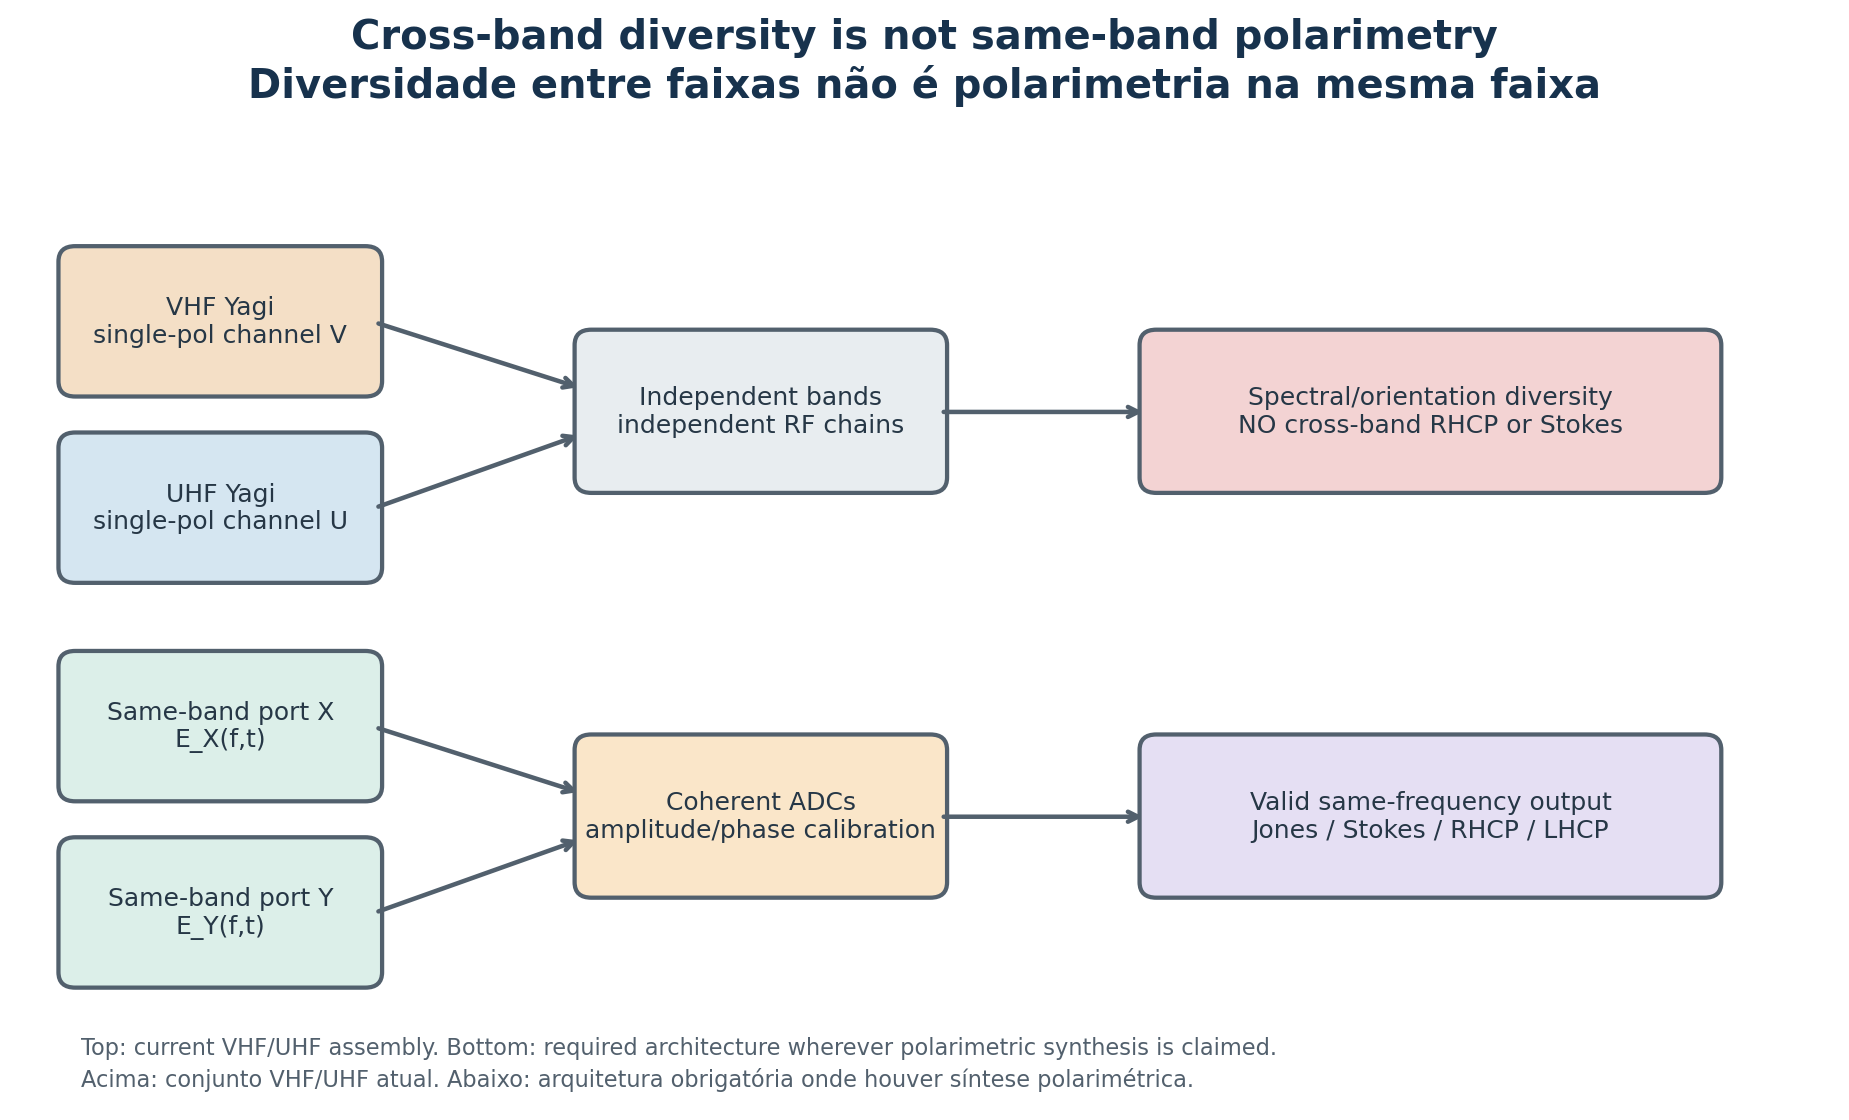
\includegraphics[width=0.98\textwidth]{fig05_polarimetria.png}
\caption{Aquisição por duas portas ortogonais e síntese digital de estados de polarização.}
\label{fig:polarimetria}
\end{figure}

\chapter{Arquitetura eletrônica distribuída}

O \vthree\ eletrônico é hierárquico. Cada banda possui antena, front-end, ADC, ASIC/FPGA e memória local. Os eventos são combinados por um ASIC de fusão da face, e somente então seguem pela fibra para os processadores centrais redundantes.

\begin{figure}[H]
\centering
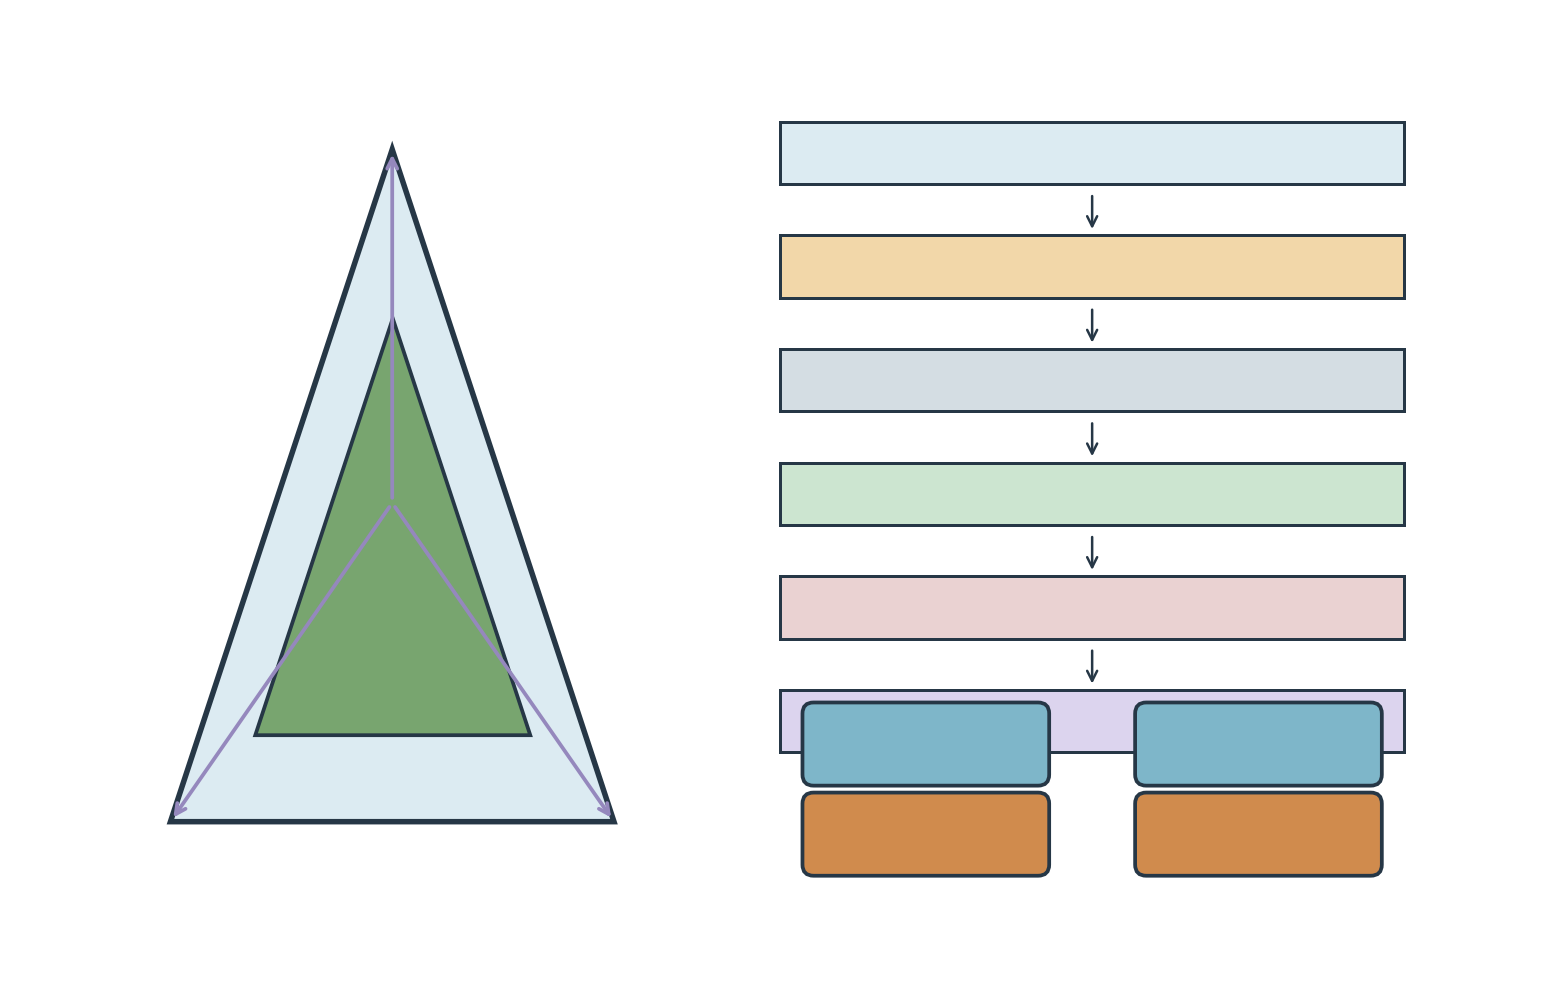
\includegraphics[width=0.98\textwidth]{fig03_modulo_face.png}
\caption{Módulo triangular de face, camadas dielétricas, plano RF, front-end, dissipação e fibra.}
\label{fig:modulo}
\end{figure}

A cadeia de uma subfaixa é:
\[
\text{antena}\rightarrow\text{pré-seletor}\rightarrow\text{limitador/LNA}\rightarrow\text{conversão}\rightarrow\text{ADC}\rightarrow\text{DDC/PFB/FFT}\rightarrow\text{detector}\rightarrow\text{evento}.
\]

O processamento local pode calcular potência, espectro, frequência central, largura de banda, SNR, duração, impulsividade, periodicidade, polarização, correlações e classificação preliminar.

\begin{figure}[H]
\centering
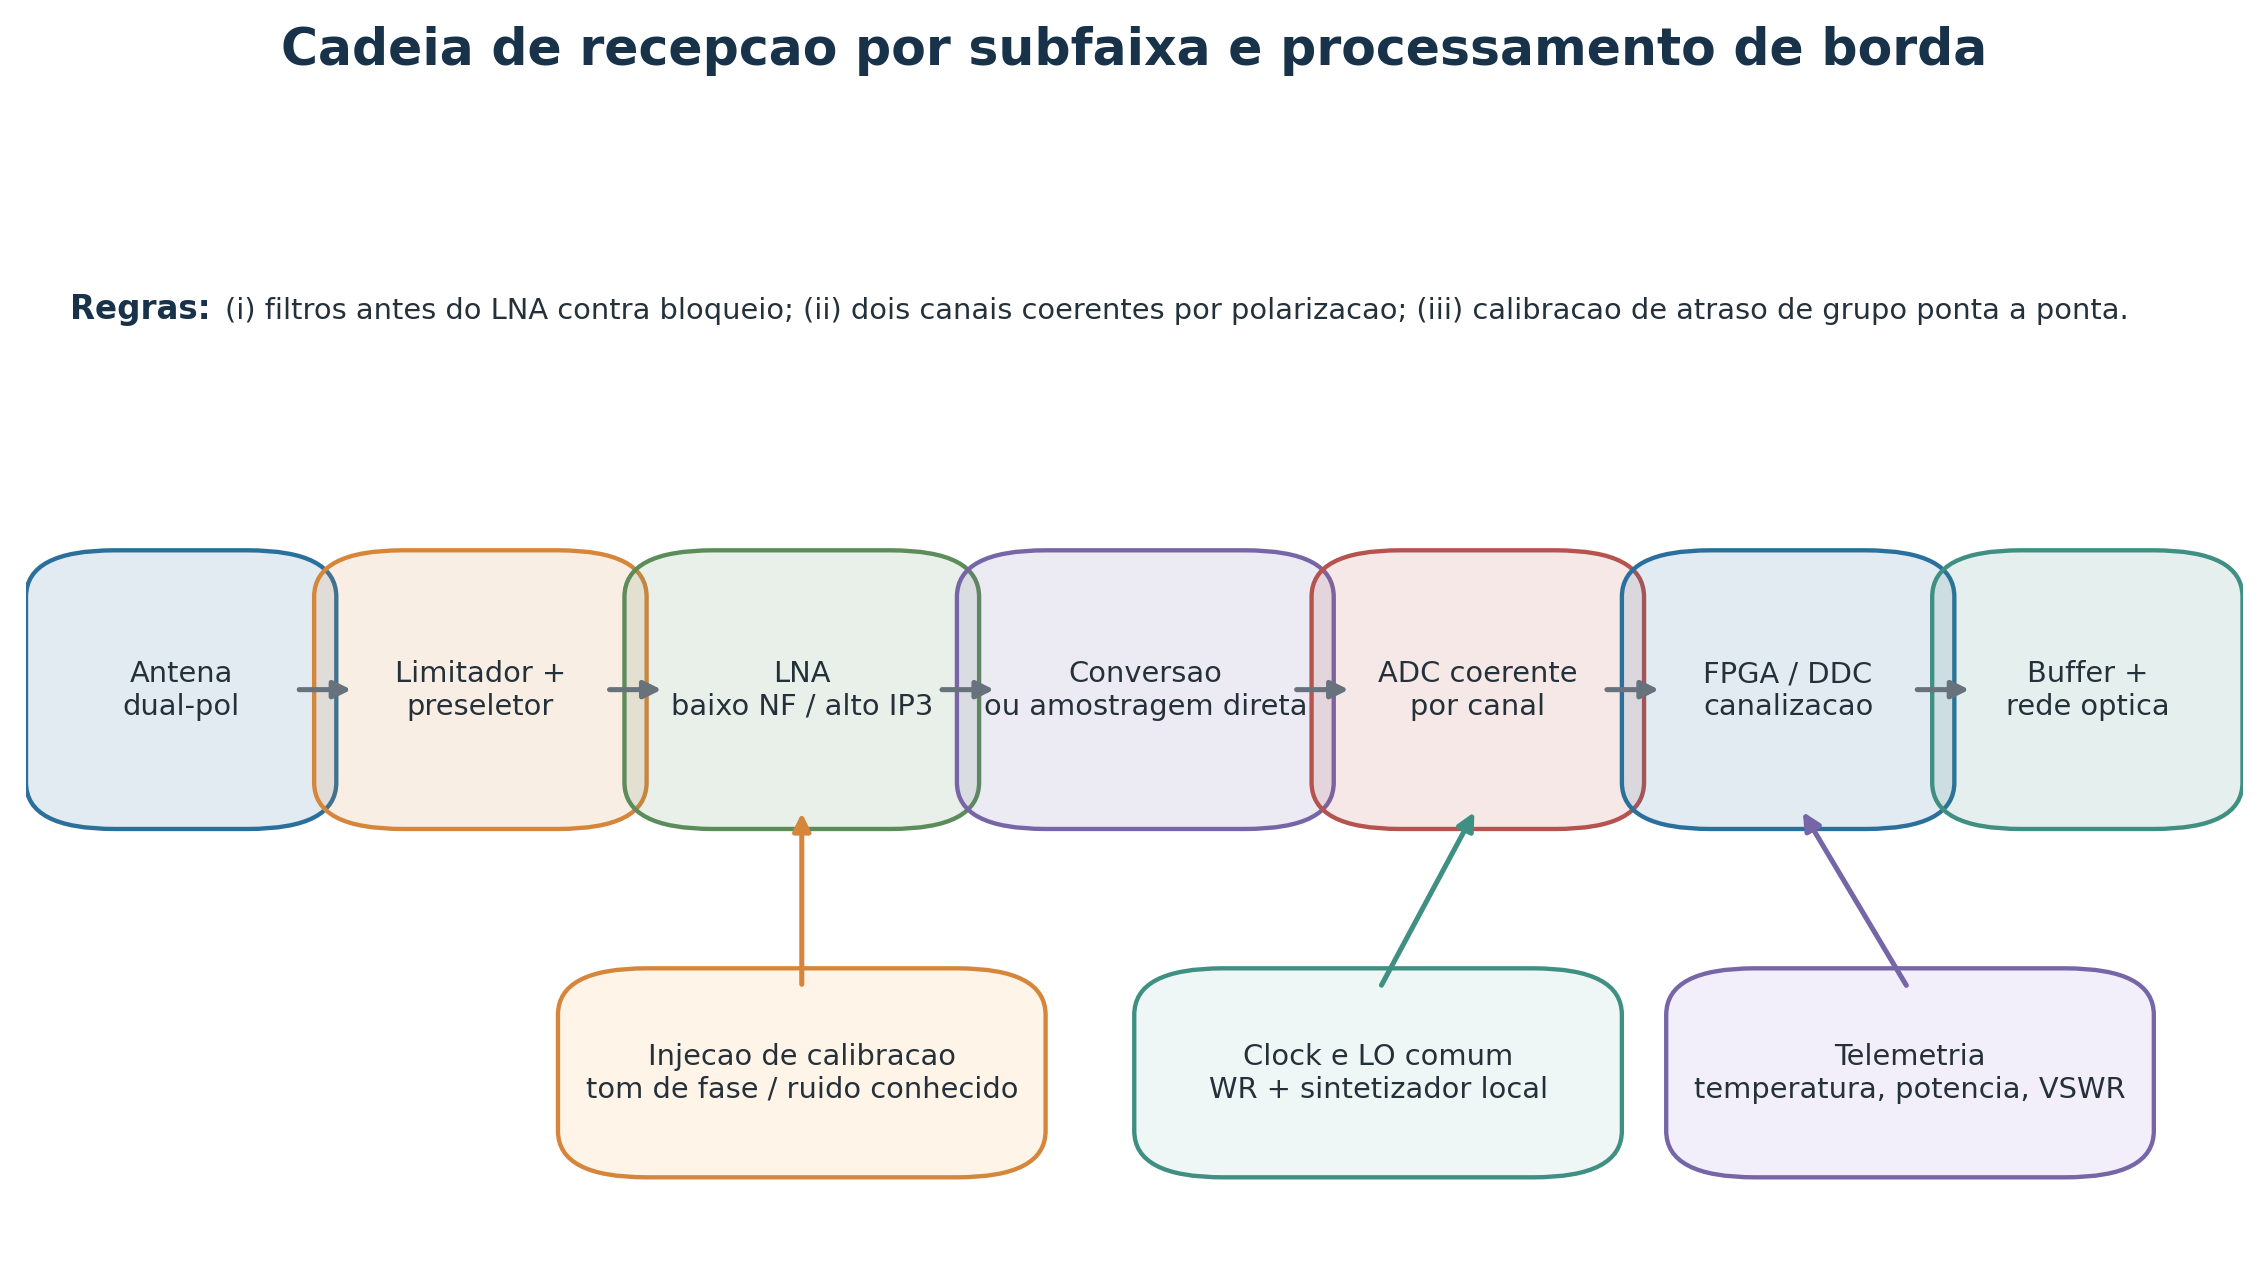
\includegraphics[width=0.98\textwidth]{fig06_cadeia_rf.png}
\caption{Cadeia RF por subfaixa, com calibração, clock, processamento e telemetria.}
\label{fig:cadeia}
\end{figure}

\section{Buffers e eventos}

Cada cadeia mantém um buffer circular. Para uma taxa de amostragem $f_s$, $b$ bits por amostra e duração $T_b$, a memória aproximada é:
\[
M_i=\frac{f_s b T_b}{8},\qquad M_{\mathrm{face}}=\sum_i M_i.
\]
Ao detectar um evento em $t_0$, preserva-se a janela $[t_0-T_{\mathrm{pre}},t_0+T_{\mathrm{post}}]$. O descritor deve conter timestamp, frequência, largura de banda, potência, SNR, polarização, confiança, estado de sincronismo e referência para o bloco bruto local.

A taxa de rede normal é orientada a eventos:
\[
R_{\mathrm{rede}}=R_{\mathrm{alertas}}+R_{\mathrm{telemetria}}+R_{\mathrm{resumos}}+R_{\mathrm{capturas}}.
\]
A capacidade interna de ADC não deve ser confundida com tráfego permanente.

\section{Hierarquia V3}
\begin{enumerate}
\item ASIC da banda: decide se há sinal potencialmente relevante;
\item FFASIC da face: correlaciona bandas, polarizações e tempos da mesma direção;
\item RASIC redundante: correlaciona as 60 faces e produz a fusão global.
\end{enumerate}

Para $N_B$ bandas por face, o número mínimo de antenas e cadeias principais é $60N_B$, além de 60 FFASICs e pelo menos dois RASICs. Para $N_B=8$, isso corresponde a pelo menos 480 antenas específicas, 480 cadeias ADC, 480 processadores de banda, 60 processadores de fusão local e dois processadores centrais redundantes.

\chapter{Sincronização e calibração}

White Rabbit ou IEEE 1588 HA pode distribuir tempo e frequência de forma determinística em fibra, mas não substitui a coerência de portadora, a calibração de atraso ou o controle de fase. O núcleo temporal deve incluir referência atômica ou oscilador de alta estabilidade, grandmaster, distribuição óptica, clock cleaner local e timestamping em hardware.

A relação entre incerteza temporal e fase é:
\[
\sigma_\phi=2\pi f\sigma_t.
\]
A \SI{30}{GHz}, uma incerteza de \SI{1}{ps} corresponde a aproximadamente 10,8 graus. Logo, beamforming intersite em Ka exige sintetizadores de baixo ruído, distribuição óptica de frequência e calibração, não apenas PPS.

Cada amostra deve ser associada a uma época comum:
\[
t_{i,j,n}=T_{\mathrm{epoch}}+\frac{n}{f_{s,i,j}}+\delta_{i,j},
\]
onde $\delta_{i,j}$ representa o atraso calibrado da cadeia. O atraso de cada canal deve ser medido como $\tau_i(f,T)$ e aplicado ao timestamp corrigido:
\[
t_i^\ast=t_i-\tau_i(f,T).
\]

\begin{figure}[H]
\centering
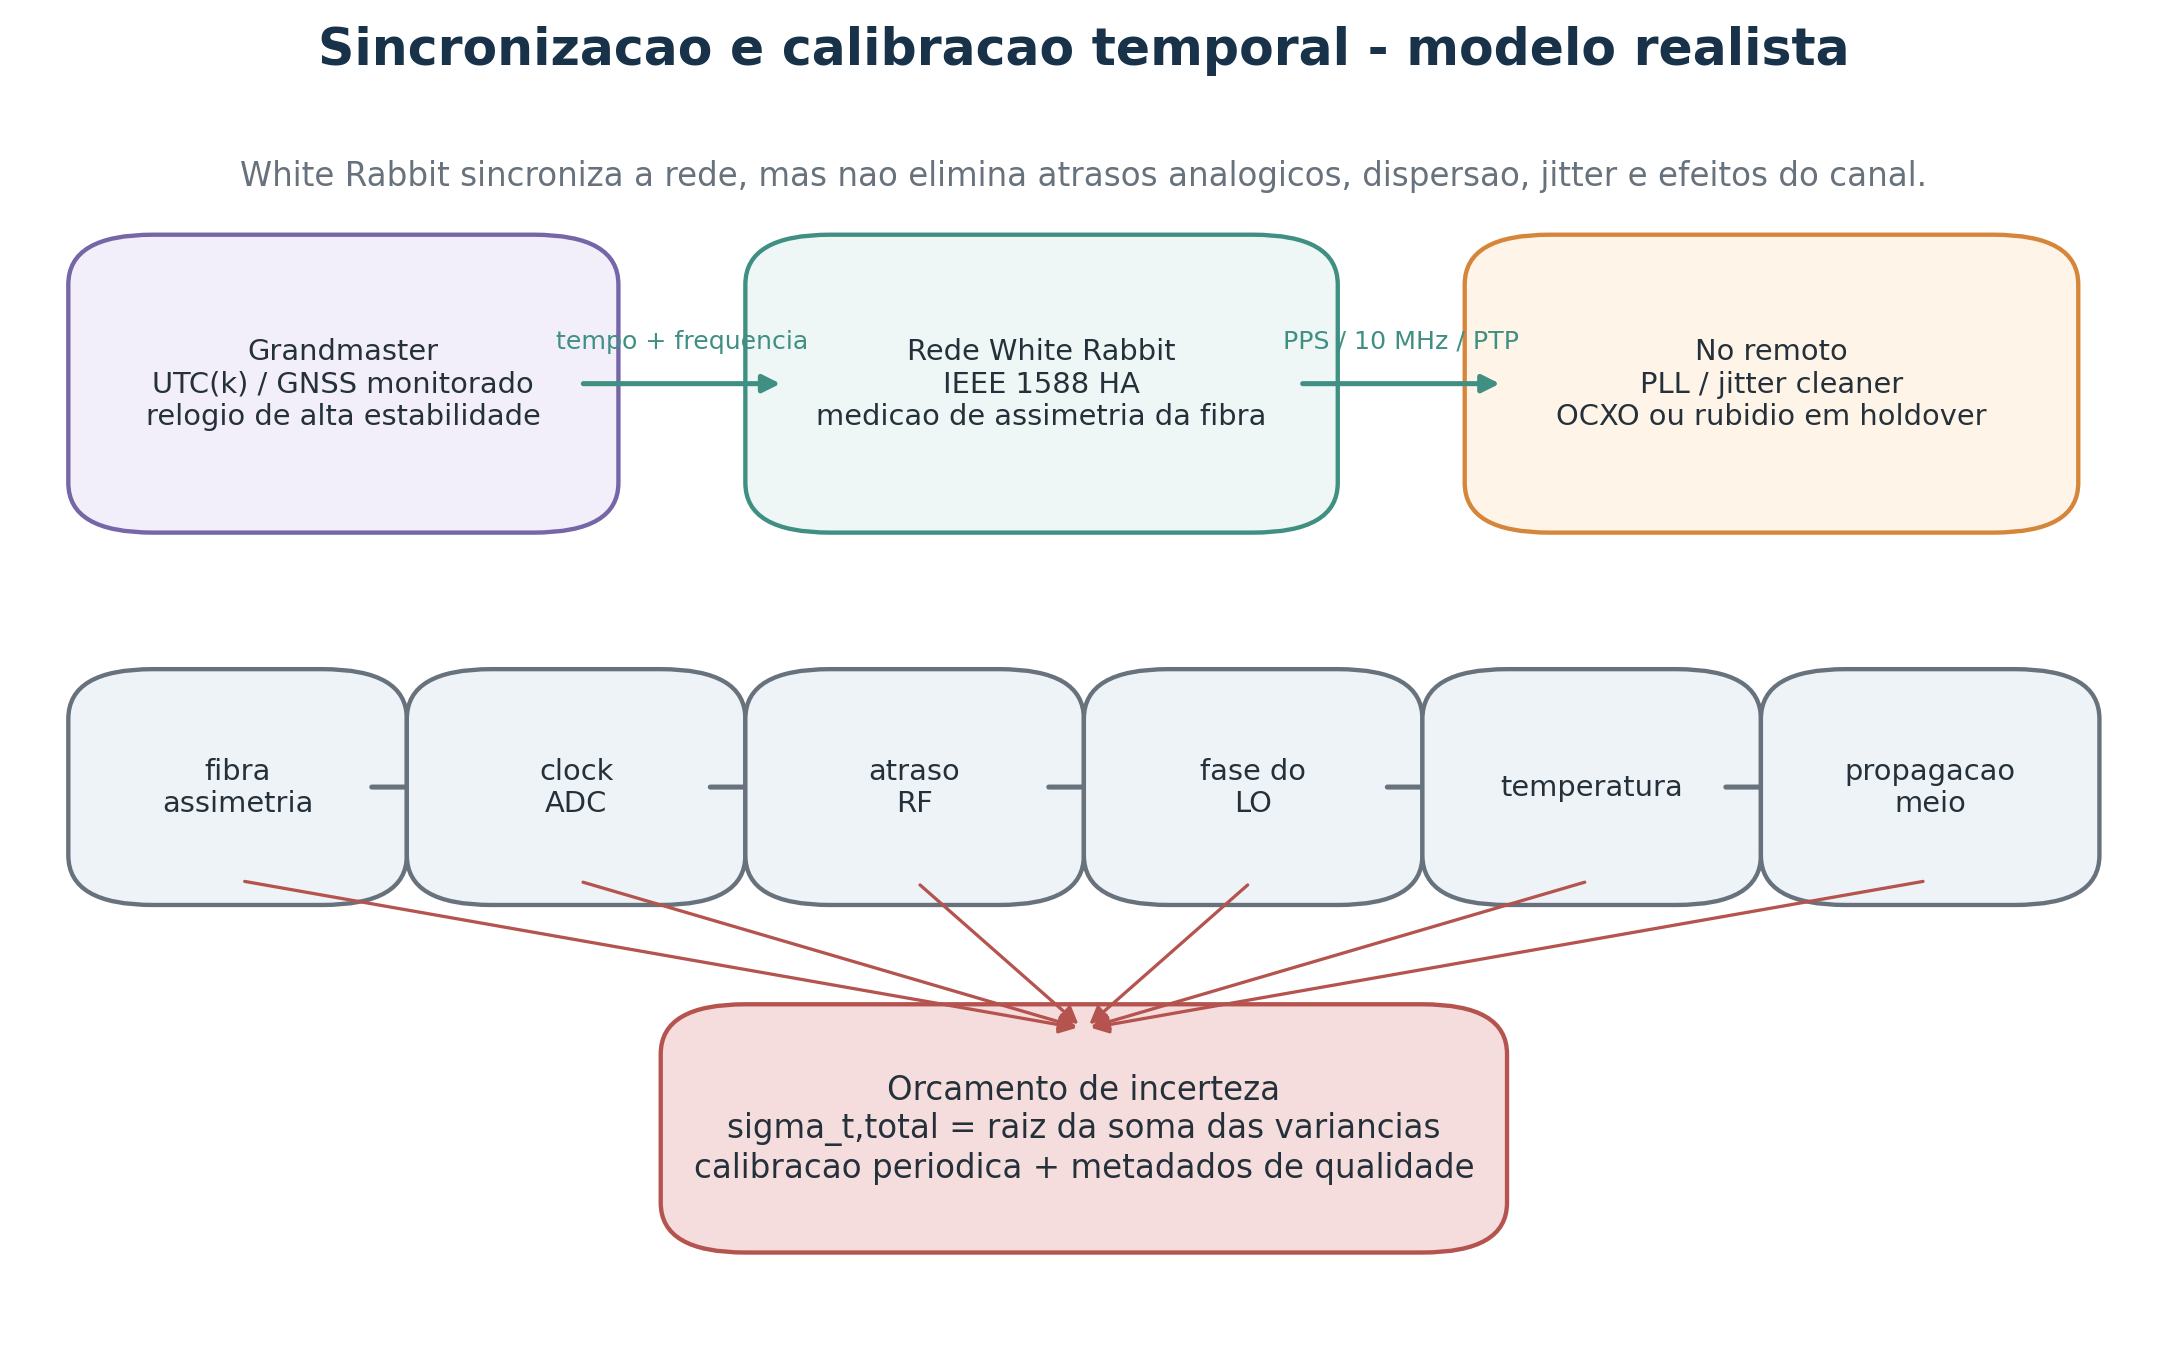
\includegraphics[width=0.98\textwidth]{fig07_sincronizacao.png}
\caption{Referência temporal, distribuição White Rabbit e orçamento de incerteza.}
\label{fig:sincronizacao}
\end{figure}

\chapter{Geometria de localização e radar passivo}

Para iluminador $T$, alvo $x$ e receptor $R_i$, o excesso de caminho bistático é:
\[
\Delta\rho_i=\lVert x-T\rVert+\lVert x-R_i\rVert-\lVert T-R_i\rVert=c\Delta\tau_i.
\]
Cada medida ideal define uma elipsoide. Para emissor direto, TDOA define hiperboloides. FDOA adiciona informação de velocidade relativa, enquanto AOA fornece linhas ou cones de direção. A fusão deve utilizar covariâncias, incerteza do iluminador, sincronismo, propagação e geometria.

\begin{figure}[H]
\centering
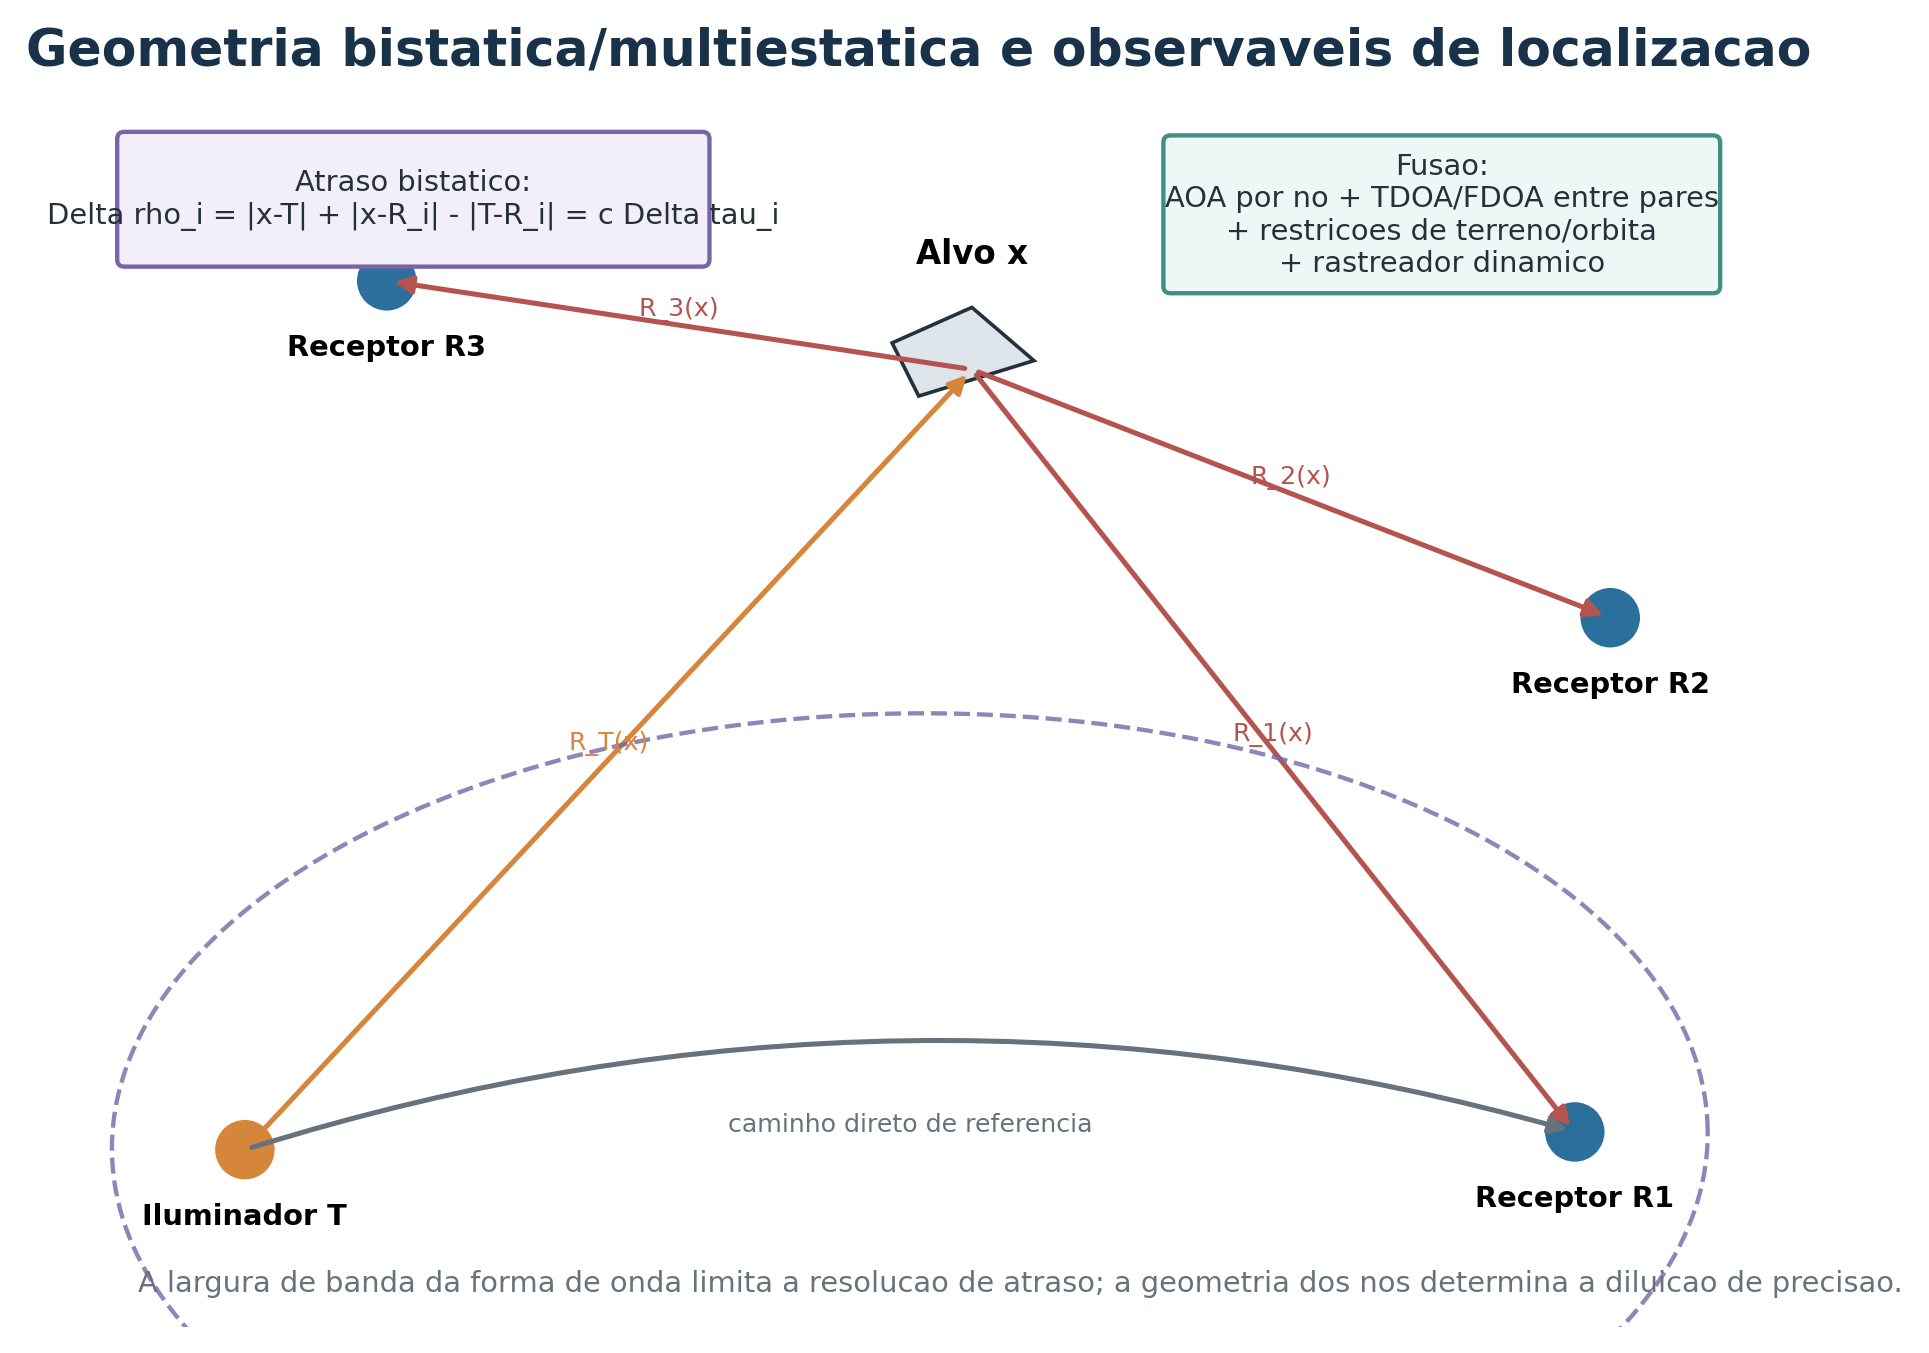
\includegraphics[width=0.98\textwidth]{fig08_geometria_bistatica.png}
\caption{Geometria bistática e observáveis utilizados na fusão multiestática.}
\label{fig:bistatica}
\end{figure}

O processamento de radar passivo começa com equalização de referência e vigilância, cancelamento do sinal direto e do clutter, função de ambiguidade cruzada e detecção com controle de falso alarme. As detecções são associadas por tempo, frequência, Doppler e consistência geométrica.

\begin{figure}[H]
\centering
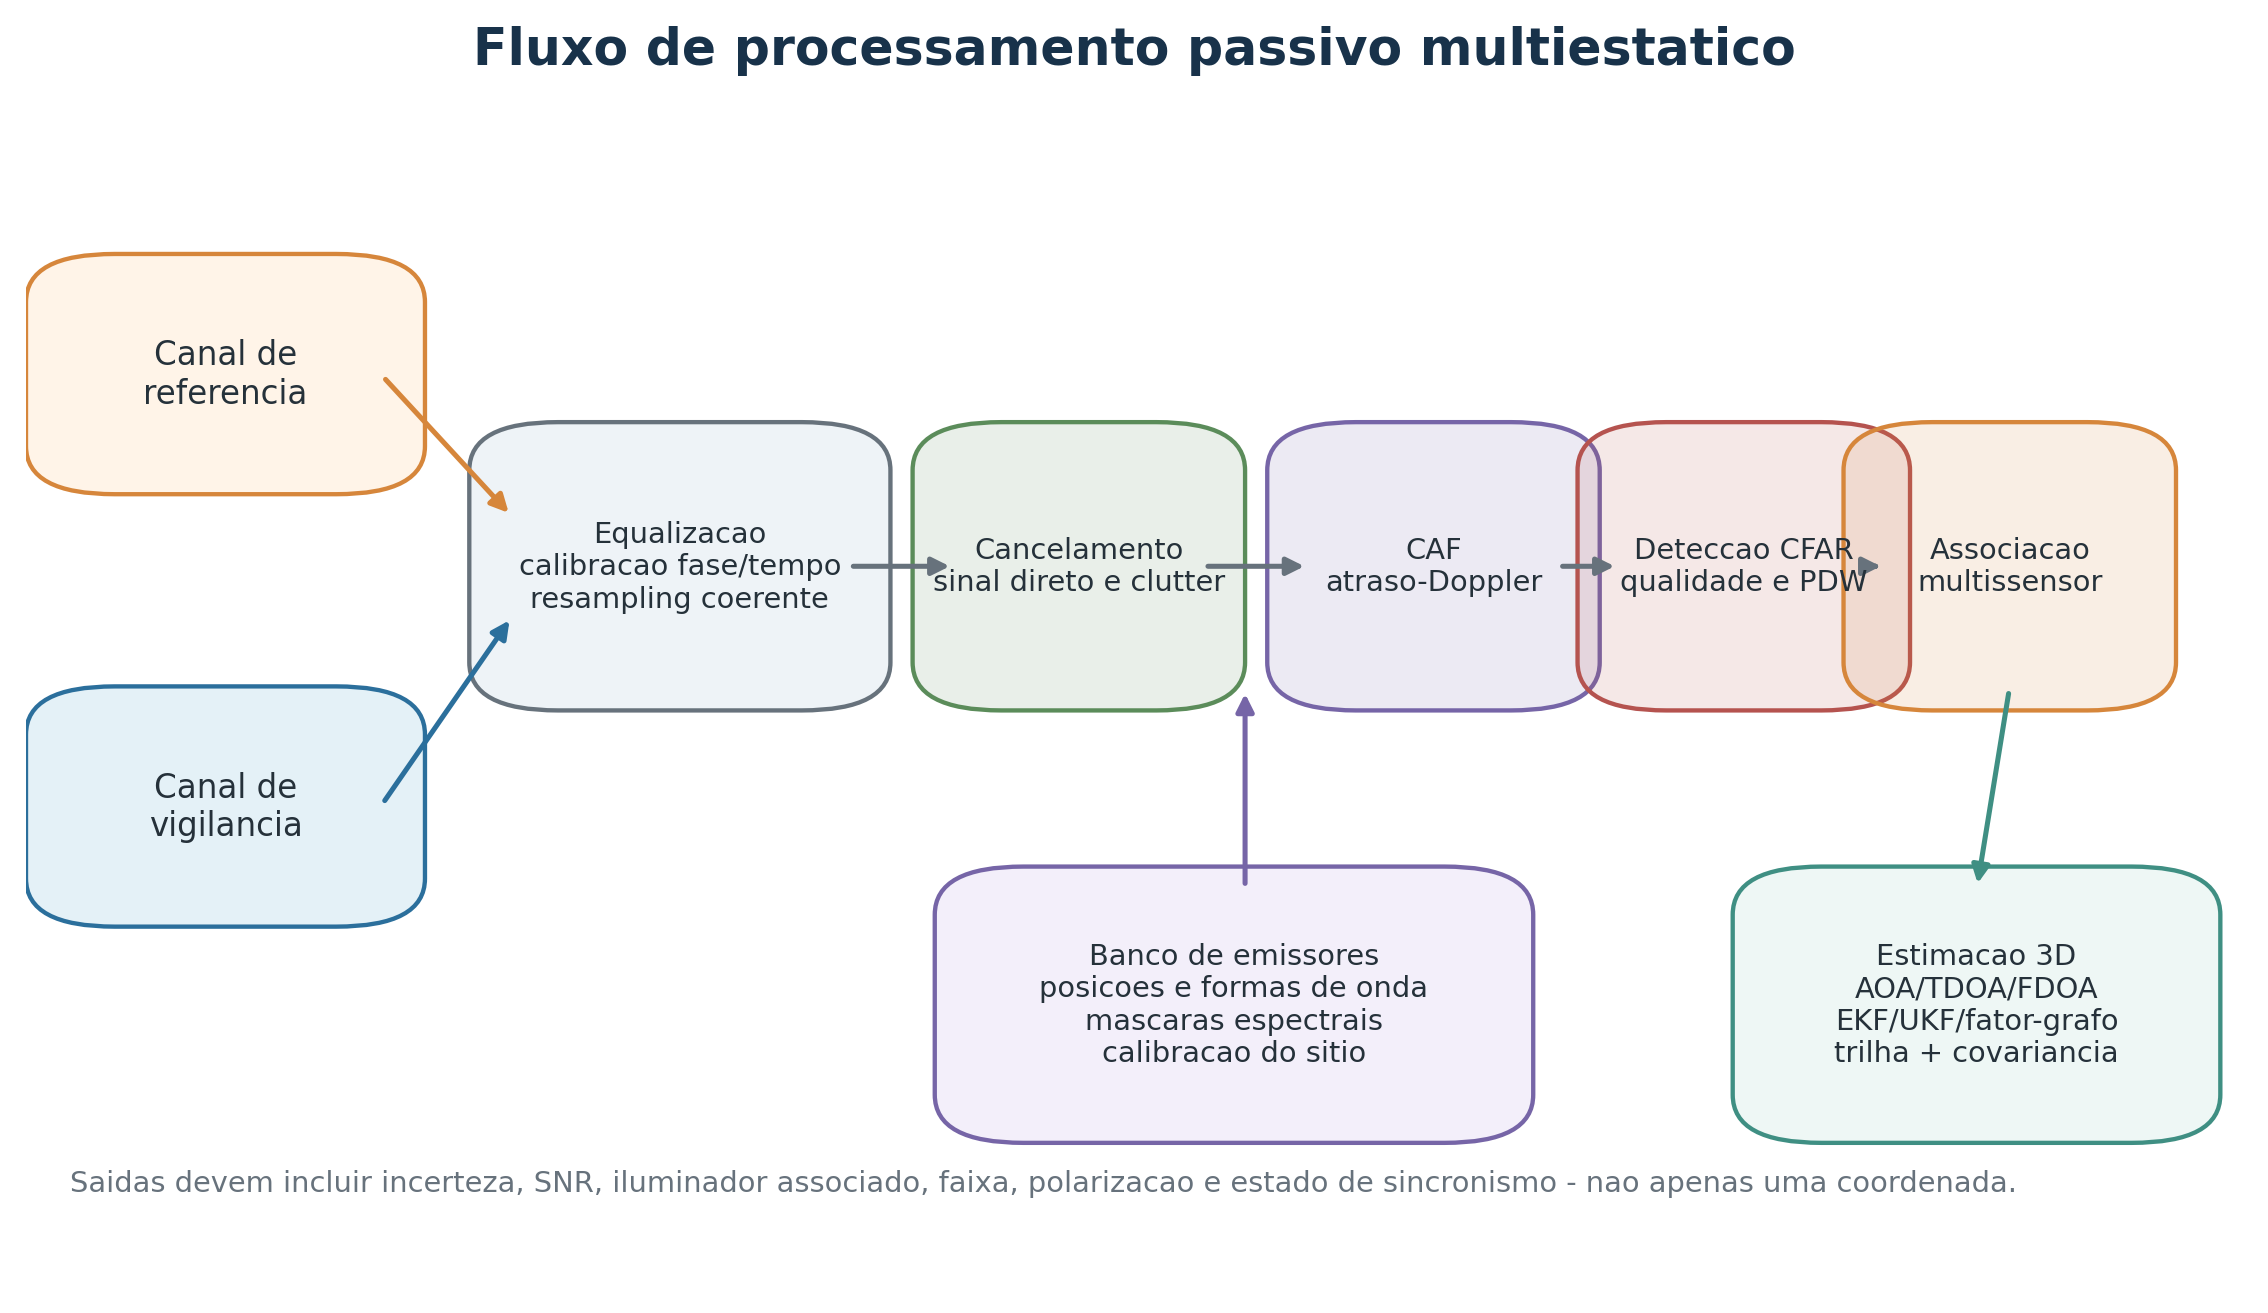
\includegraphics[width=0.98\textwidth]{fig09_fluxo_processamento.png}
\caption{Fluxo de referência e vigilância até uma trilha tridimensional com covariância.}
\label{fig:processamento}
\end{figure}

\chapter{Infraestrutura de alta montanha}

O plano diretor associado ao projeto acrescenta a infraestrutura necessária à operação de uma estação: centro de supervisão, energia híbrida, UPS, banco de baterias, gerador, fibras redundantes, climatização, proteção contra descargas, segurança perimetral e logística de heliponto. Esses elementos devem ser tratados como parte do sistema, pois energia, temperatura, vibração e EMI afetam diretamente a metrologia RF.

A arquitetura de energia recomendada utiliza rede principal, ATS, gerador, UPS de dupla conversão, bateria LiFePO$_4$, barramento DC e distribuição seletiva. A fibra deve possuir dutos próprios e permanecer fisicamente separada dos circuitos de potência. O complexo deve incluir sensores optrônicos e sistemas de segurança compatíveis com a operação de receptores sensíveis.

\section{Requisitos ambientais e EMC}
\begin{itemize}
\item vento, vibração, chuva, UV, umidade, salinidade e variação térmica;
\item dissipação térmica dos tiles e controle de condensação;
\item blindagem compartimentada e filtros feedthrough;
\item proteção contra descargas sem criar uma gaiola metálica contínua sobre as aberturas;
\item redundância de energia, dados e sincronismo;
\item avaliação de relevo, horizonte, RFI local, acesso e disponibilidade de fibra antes da seleção do sítio.
\end{itemize}

\chapter{Revisão de literatura, inovação e lacunas}

A revisão bibliográfica mostra três linhas relativamente maduras, mas pouco integradas: antenas e arrays conformais; radomes funcionais e FSS; e processamento de sinais para detecção, direção e identificação de emissores. Trabalhos sobre arrays conformais enfatizam que acoplamento mútuo, estrutura e radome fazem parte do manifold calibrado, não sendo suficiente especificar apenas perda de retorno e ganho \citep{caratelli2011,liberal2011}.

A literatura de radomes seletivos mostra soluções com transmissão em banda e absorção ou difusão fora de banda \citep{costa2012,lv2021,omar2018,sheng2024}. Para uma rede de vigilância ampla, a seletividade deve ser escolhida com cuidado: uma solução concebida para absorver emissões fora de uma banda pode ser incompatível com monitoramento aberto do espectro.

A literatura de localização passiva utiliza AOA, TDOA e FDOA, com forte dependência da geometria, sincronismo e carga computacional \citep{liu2019,pine2021}. Métodos de fingerprinting e detecção aberta podem auxiliar a caracterização de emissores desconhecidos, mas classificadores fechados e modelos treinados em condições limitadas não devem ser apresentados como solução universal \citep{soltanieh2020,jagannath2022,sun2022}.

A lacuna do projeto é a integração de abertura conformal multifaixa, recepção passiva distribuída, calibração polarimétrica e temporal, processamento hierárquico e validação em ambiente montanhoso realista. A inovação é sistêmica e deve ser demonstrada por medições reproduzíveis, não apenas por diagramas ou simulações isoladas.

\chapter{Plano de prototipagem e aceitação}

\begin{longtable}{p{0.18\textwidth}p{0.38\textwidth}p{0.32\textwidth}}
\toprule
\textbf{Fase} & \textbf{Entrega} & \textbf{Gate de validação}\\
\midrule
P0 & requisitos, cobertura, orçamento de enlace e incerteza & hipóteses rastreáveis e riscos dominantes identificados\\
P1 & três nós VHF/UHF, canais de referência e vigilância & localização de emissor cooperativo e alvo de teste\\
P2 & tile L/S/C, polarimetria e painel de radome & VSWR ativo, ganho, AR e varredura medidos\\
P3 & tiles X/Ku/Ka, LO de baixo jitter e térmica & feixe e polarização preservados na faixa especificada\\
P4 & demonstrador integrado e campanha externa & falso alarme, disponibilidade e covariância documentados\\
\bottomrule
\end{longtable}

Os ensaios devem incluir S-parâmetros, padrão 3D OTA, perda e fase do radome, coerência de canais, offset/jitter/TDEV/holdover, AOA calibrado, cancelamento do sinal direto, Pd/Pfa e recuperação após perda de fibra ou energia.

\begin{figure}[H]
\centering
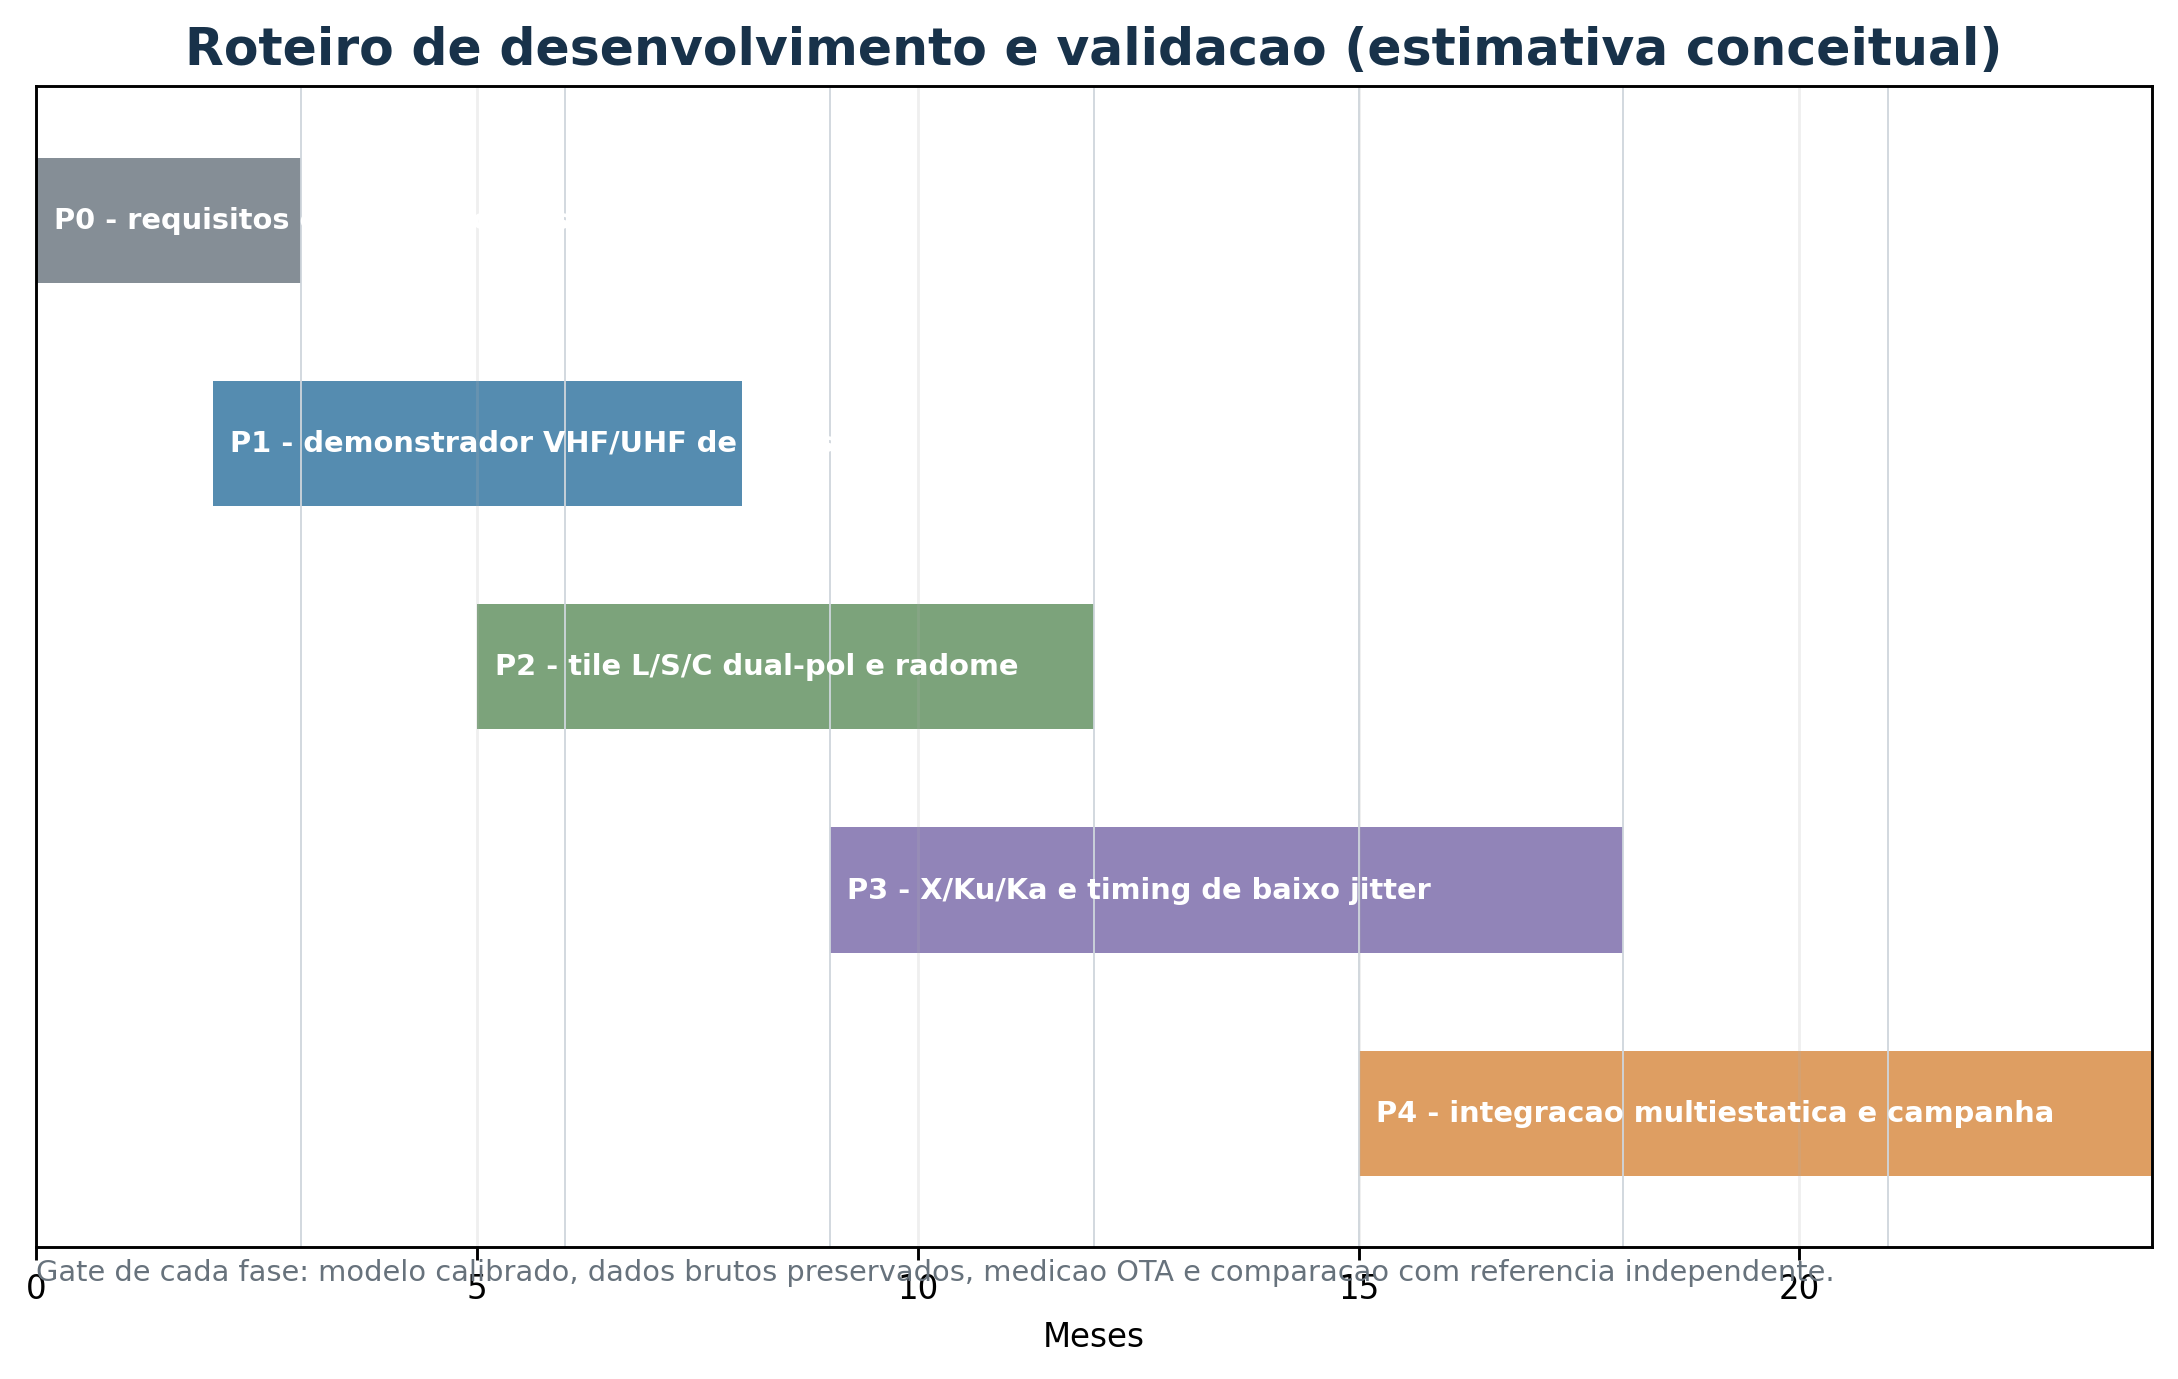
\includegraphics[width=0.98\textwidth]{fig10_roteiro.png}
\caption{Roteiro conceitual de desenvolvimento e validação.}
\label{fig:roteiro}
\end{figure}

\chapter{Riscos e limites}

Os principais riscos são saturação por emissores locais, acoplamento entre bandas, deriva térmica, modelo ideal de antena, vazão excessiva, propagação não livre, radome molhado ou envelhecido e promessas de desempenho sem orçamento de enlace. As mitigações correspondentes são pré-seletores, limitadores, alto IP3, co-simulação, padrões medidos, processamento local, modelos atmosféricos, ensaios climáticos, recalibração e especificações probabilísticas.

Nenhum alcance ou precisão deve ser declarado sem informar potência e forma de onda do iluminador, distâncias, ganho, temperatura de sistema, perdas, integração, seção radar bistática, geometria e probabilidades de detecção e falso alarme.

\chapter{Conclusão}

A consolidação confirma um conceito tecnicamente defensável: combinar radomes distribuídos, digitalização próxima às antenas, canais de referência e vigilância, sincronização de alta estabilidade, processamento hierárquico e fusão multiestática. A correção decisiva em relação às versões iniciais é abandonar a face universal e adotar subsistemas de escalas eletromagnéticas diferentes.

O caminho de menor risco é um demonstrador de três nós em VHF/UHF, seguido por tiles L/S/C e posteriormente por X/Ku/Ka. HF deve ser desenvolvido como programa próprio de sensores vetoriais e modos característicos. A expansão territorial só deve ocorrer depois da validação de cobertura, orçamento de enlace, geometria, falso alarme, estabilidade metrológica e desempenho ambiental.

\appendix
\chapter{Registro mínimo de detecção}
\begin{longtable}{p{0.32\textwidth}p{0.55\textwidth}}
\toprule
\textbf{Campo} & \textbf{Descrição}\\
\midrule
station\_id & identificador do nó e versão da calibração\\
tile\_id/channel\_id & tile, porta de polarização e cadeia RF\\
timestamp\_utc & tempo com incerteza estimada\\
frequency\_hz/bandwidth\_hz & centro e largura de banda\\
complex\_amplitude & I/Q ou amplitude/fase referenciada\\
polarization & Stokes ou Jones com covariância\\
aoa\_az\_el & direção local e matriz de covariância\\
delay\_doppler & medidas bistáticas e qualidade\\
illuminator\_id & identidade ou hipótese do iluminador\\
sync\_state & locked, holdover ou degraded\\
environment & temperatura, umidade e estado do radome\\
\bottomrule
\end{longtable}

\chapter{Fontes documentais consolidadas}

A síntese foi construída a partir dos seguintes documentos e materiais:
\begin{itemize}
  \item \texttt{RADOME V3.md} e \texttt{RADOME V3 -- Arquitetura Eletrônica Distribuída Revisada.md};
  \item \texttt{Projeto\_Radomes\_Multifaixa\_Revisado.md};
  \item \texttt{plano\_diretor\_complexo\_vigilancia\_alta\_montanha.md};
  \item \texttt{review.md}, \texttt{references.bib} e os documentos PDF associados;
  \item figuras técnicas em \texttt{Projeto\_Radomes\_Multifaixa\_Revisado\_Markdown/figures/}.
\end{itemize}

\bibliographystyle{plainnat}
\bibliography{references}
\end{document}
